\documentclass[main.tex]{subfiles} % Subfile-Class

% ============================================================================== %
%                            Subfile document                                    %
% ============================================================================== %

\begin{document}

% Template

\subsection{Aufgabenstellung}

Die Aufgabenstellung des Moduls Produktentwicklung PREN 1 der
Hochschule Luzern fordert uns als interdisziplinäres Team heraus, ein autonomes 
Fahrzeug zu entwickeln, das ein vorgegebenes Wegenetzwerk optimal navigieren kann. 
Das Fahrzeug soll Hindernisse erkennen, gesperrte Bereiche meiden und die kürzeste 
Route zum Ziel unter Berücksichtigung unbekannter Einschränkungen finden.

Unser Team aus Studierenden der Elektrotechnik, Informatik und Maschinenbau 
vereint verschiedene technische Kompetenzen. In der Projektphase von PREN 1 
entwickeln wir ein Gesamtkonzept basierend auf einem morphologischen Kasten, 
um Lösungsvarianten systematisch zu vergleichen. Dabei bewerten wir die technische 
Machbarkeit und erstellen erste Prototypen als Grundlage für das Modul PREN 2.

Zu den wichtigsten Anforderungen zählen:
\begin{itemize}
    \item \textbf{Erkennung gesperrter Wegpunkte:} Pylonen müssen selbstständig detektiert werden.
    \item \textbf{Bewältigung von Hindernissen:} Hindernisse sollen aktiv entfernt und zurückgestellt werden.
    \item \textbf{Anpassung an veränderte Bedingungen:} Fehlende Streckenabschnitte müssen als nicht passierbar erkannt werden.
    \item \textbf{Autonome Zielfindung:} Über eine Zielauswahl vor dem Start soll das Fahrzeug die effizienteste Route finden.
\end{itemize}

Zudem werden bei der Umsetzung strenge Vorgaben zu Dimensionen, Gewicht und
Autonomie des Systems berücksichtigt. Dies umfasst die Integration sämtlicher
Hardware-Komponenten in das Fahrzeug sowie die Sicherstellung eines
störungsfreien und sicheren Betriebs. Weiterhin erarbeiten wir in PREN 1 erste
Simulationen, die das Verhalten des Systems unter realitätsnahen Bedingungen
analysieren und optimieren.

Die wissenschaftliche Herausforderung besteht darin, Sensorik, Elektronik 
und Algorithmen so zu kombinieren, dass eine zuverlässige Wegfindung und 
Hindernisbewältigung gewährleistet ist. Dabei legen wir besonderen Wert auf 
eine methodische Herangehensweise, die auch Nachhaltigkeitsaspekte berücksichtigt.

Das Projekt bietet uns die Möglichkeit, theoretisches Wissen praktisch 
anzuwenden und unsere Kompetenzen in interdisziplinärer Zusammenarbeit 
und systematischer Produktentwicklung zu vertiefen.

\begin{figure}[H]
    \centering
    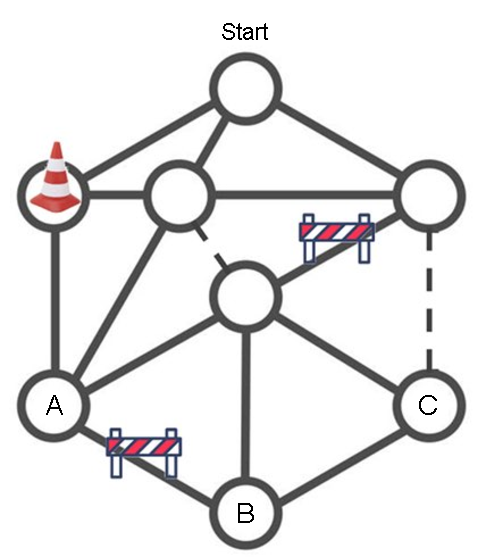
\includegraphics[width=0.25\textwidth]{Wegenetzwerk_Aufgabenstellung.pdf}
    \caption{Beispiel Wegenetzwerk aus Aufgabenstellung}~\label{fig:Wegenetzwerk_Aufgabenstellung}
\end{figure}

\end{document}